\chapter{Calibration and Characterisation}
\label{ch:characterisation}
\minitoc

    Before we can proceed with our planned experiments involving the motion and
    spin of the ions, the apparatus must be characterised. This characterisation
    serves two purposes: it allows us to benchmark the performance of our
    system, and it reveals any current limitations
    that must be addressed before we can successfully carry out the experiments.\\

    We split this chapter into interactions involving only the spin, then those
    focussed only on the motion, and finally we describe spin-motion
    interactions. This chapter demonstrates the full control required for
    discrete-variable quantum computation. Section~\ref{sec:CVQC} in
    chapter~\ref{ch:QEM} applies the spin-dependent motional
    interactions demonstrated here for continuous-variable readout, and to
    realise the remaining nonlinear and two-mode operations required
    for full hybrid CV-DV control.\\

\section{Spin}
\label{sec:Spin}
    Discrete variable quantum computing consists of control over many two-level
    systems, which we refer to either as spins, or qubits. In this section 
    the experimental methods used to prepare, manipulate, and measure these spins are described, and the
    performance of these operations are benchmarked.\\

\subsection{State Preparation}
\label{sec:Stateprep}
% Main points:
    % Method of preparation via optical pumping
    % Quote state prep error (back this from RBM + measurement histograms)
% Pre reqs:
    % Laser systems powers
    % 729 system
    % Available transitions
    % pi-pulses

    \begin{figure}
        \begin{center}
        \noindent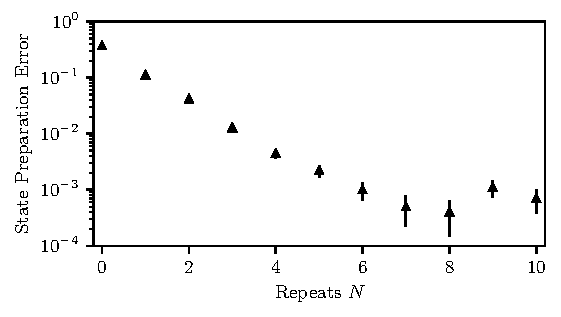
\includegraphics[width=0.667\linewidth]{
            figures/pdf_figure/ch4/state_prep.pdf
            }
        \end{center}
        \caption{
            State preparation error as a function of the number of state preparation pulses, $N$. The error is defined as population not in the $\ket{\downarrow}$ state after the preparation sequence has been applied. The error is reduced to below $10^{-3}$ after $N=7$ pulses, which is used in our experiments.
            }
        \label{fig:stateprep}
    \end{figure}

\begin{table}
    \begin{center}
    \begin{tabular}{|c|l|}
        \hline
        Parameter & Value \\
        \hline
        729-nm laser power & 1000~\unit{\uW}\\
        729-nm pulse duration & 5~\unit{\us} \\
        854-nm laser power & 60~\unit{\uW}, $250\times I_{\rm SAT}$\\
        854-nm pulse duration & 40~\unit{\us} \\
        866-nm laser power & 15~\unit{\uW}, $\sim 70\times I_{\rm SAT}$\\
        866-nm pulse duration & 30~\unit{\us} \\
        \hline
    \end{tabular}
    \end{center}
    \caption{
        Experimental parameters used for state preparation of the ion into the $\ket{\downarrow} = \ket{4S_{1/2},~m_j = -1/2}$ state. All lasers frequencies are set to be resonant with the corresponding transition frequencies.
        }
    \label{tab:state_prep_parameters}
\end{table}

    To utilise two levels of the ion as a qubit, the electronic state must first be prepared into the qubit manifold. Here, the ion is prepared into the $\ket{\downarrow}=\ket{4S_{1/2},~m_j=-1/2}$ state. 
    This is done via optical pumping by pulsing the quadrupole transition $\ket{4S_{1/2},~m_j = +1/2} \leftrightarrow \ket{3D_{5/2},~m_j = -3/2}$,
    followed by deshelving pulses using the 854-nm, 866-nm
    lasers on resonance.  The 729-nm laser pulse duration and intensity is set to invert the populations, i.e. perform a $\pi$-pulse. Details for laser parameters are summarised in Table~\ref{tab:state_prep_parameters}. These three pulses are repeated $N$ times sequentially. Figure~\ref{fig:stateprep} shows the state preparation error with increasing $N$. The error is found by applying a $\pi$-pulse on the state preparation transition directly after the state preparation sequence and measuring the population in the $\ket{\downarrow}$ state, $P_\da$. Any population not in $P_\da$ indicates either residual population in the $\ket{4S_{1/2},~m_j = +1/2}$ state, or trapped in the metastable $D$ levels. After $N=7$ pulses there is a state preparation error of $<10^{-3}$. The state preparation error is likely limited by accidental excitation of the $\ket{4S_{1/2},~m_j = -1/2}$ state to the $D_{5/2}$ level. This may be due to off-resonant excitation of another transition, or due to spectral purity of the 729-nm laser. \\


\subsection{Measurement}
\label{sec:Measurement}
% Main points:
    % Readout characterisation with NA 0.6 lens
    % Compare readout histograms of fast 30 us readout to Doppler cold 100 us readout
    \begin{figure}
        \begin{center}
        \noindent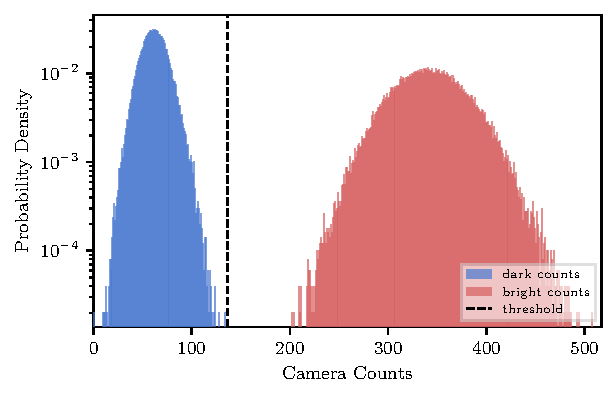
\includegraphics[width=0.75\linewidth]{
            figures/pdf_figure/ch4/readout_hist.pdf
            }
        \end{center}
        \caption{
            Readout histogram with 100,000 individual measurements for bright (red) and dark (blue) populations. The camera counts are presented as a histogram and fitted to Poissonian distributions to calibrate a threshold for discerning if the ion is bright or dark with the lowest probability for false measurement. Dark counts are mainly due to 397-nm light scattered from the nearest trap electrodes. With 100~\unit{\us} readout duration, and laser parameters set to Doppler cooling parameters, a threshold of 137 photons is found to be sufficient to discern the two populations.
            }
        \label{fig:readout_histogram}
    \end{figure}

    \begin{table}
        \begin{center}
        \begin{tabular}{|c|l|}
            \hline
            Parameter & Value \\
            \hline
            397-nm laser power & 3~\unit{\uW}, $1\times I_{\rm SAT}$ \\
            397-nm laser detuning & -17.5~\unit{\MHz}\\
            866-nm laser power & 15~\unit{\uW}, $\sim 70\times I_{\rm SAT}$\\
            866-nm laser detuning & 0~\unit{\MHz} \\
            Doppler cooling duration & 1~\unit{\ms}\\
            Readout duration & 100~\unit{\us} \\
            Camera threshold & 137 counts \\
            \hline
        \end{tabular}
        \end{center}
        \caption{
            Experimental parameters used for Doppler cooling and state-selective fluorescence of the ion. 
            }
        \label{tab:397_parameters}
    \end{table}

    To measure the qubit state, the 397-nm and 866-nm lasers
    are applied, and the scattered 397-nm photons are imaged by the objective onto a camera (see~\S~\ref{sec:Imaging System}). 397-nm light will only be scattered if the qubit is in $\ket{\downarrow}$.
    A typical image generated by the camera is seen in Figure~\ref{fig:readout}. A small window of pixels in set around each ion (typically a $3\times3$ px region), and the photon counts in this region are summed.  
    Use of a high numerical aperture (NA = 0.6) objective greatly increases the collection efficiency.
    This efficiency allows the 397-nm beam to be red-detuned to Doppler cooling parameters (see~\S~\ref{sec:Cooling}), while still maintaining low readout duration (100~\unit{\us}) and low readout error. 
    Cooling during readout increases the experiment's repetition rate by reducing the amount of dedicated cooling time required.\\
    The parameters used for readout are
    summarised in Table~\ref{tab:397_parameters}, and a typical histogram of
    readout counts for one ion can be seen in
    Figure~\ref{fig:readout_histogram}. The readout threshold is calibrated by taking bright counts with the 397-nm and 866-nm lasers on, and dark counts with the 397-nm laser on and the 866-nm laser off. This assumes dark counts are due to 397-nm scattering from the trap electrodes. 
    Fitting Poissonian distributions to the bright and dark measurements, an optimal count threshold of
    is determined, shown by black dashed line. Assuming Poissonian statistics this threshold would give an expected
    statistical readout error of $\epsilon_\downarrow = \epsilon_\uparrow = 6\times10^{-9}$, where $\epsilon_{\downarrow,\uparrow}$ are the expected error associated with measuring bright or dark. This measurement ignores errors due to the
    finite lifetime of the metastable $3D_{5/2}$ level, which dominate $\epsilon_\uparrow$. The expected error due
    to the finite lifetime, $\tau$, is $\epsilon_{\rm decay} = 1 - e^{-t/\tau}$, where $t$ is the readout duration. For \ca, $\tau \sim 1.1$~s, $\epsilon_\uparrow \approx \epsilon_{\rm decay}  = 
    10^{-4}$. 
    Assuming the metastable lifetime is limited only by spontaneous decay overlooks leakage from the 854-nm deshelving beam, which could significantly shorten $\tau$~\cite{sotirova_high-fidelity_2024}. Further characterisation of the combined state-preparation and measurement fidelity is provided in~\S~\ref{sec:standard_rb}.


\subsection{Single-Qubit Rotations}
\label{sec:Single Qubit Gates}
% Main points:
    % Here is a characterisation of single qubit gates.
    % Explain RBM method
    % Quote values measured
    % What is likely error source
    % Are we limited by this error?
    % What is state of the art (for optical quadrupole transition)
    % What contribution is the spin coherence time?
% Pre reqs:
    % Spin coherence times
    % Possible transitions
    % Calibrating gate times

Single-qubit rotations driven by optical fields, as described in~\S~\ref{sec:Rabi Flopping}, along with two-qubit gates are required for universal discrete variable quantum computation. \\

We divide errors affecting single-qubit gates into two categories: unitary, and non-unitary. The unitary error component is labelled ``systematic'' if there exists simple (and accessible) control parameters to suppress such errors. 
We outline in the next section robust phase estimation (RPE), the calibration routine used to reduce systematic errors. 
In contrast, reducing non-unitary errors require improved isolation between the qubit and environment, or suppressed noise on the single-qubit-driving field. At the end of this section we characterise the performance of the single-qubit gates using randomised benchmarking.

\subsubsection{Robust Phase Estimation}
\label{sec:RPE}

Many gate calibrations can be formulated as phase estimation tasks. A
single-qubit rotation may be generally represented by $R_{\vec n}(\theta)$,
where $\vec n$ is some given axis around which the state evolves with rotation
angle $\theta=\omega t$, where the angle is accumulated over time by rate
$\omega$. For a gate we specify this axis and total angle, with deviations to the
ideal setting being a systematic error.\\
Suppose we can set axis $\vec n$, and
the interaction duration $t$ arbitrarily well, the task of calibration is then
limited to how precisely we can measure $\omega$. We further assume some
statistical uncertainty for a practical phase measurement, $\sigma_\theta$, that is
independent of the magnitude of $\theta$.
The uncertainty of angular frequency $\sigma_\omega=\frac{\sigma_\theta}{t}$ is thus 
inversely proportional to duration $t$ --- longer probe durations provide 
more information. This improved signal to noise is understood by the coherent
accumulation of phase over time due to an underlying $\omega$.\\
However, there
are two issues with going to large $t$: first, incoherent errors also
accumulate, attenuating the measured signal, and violating our assumption of a
fixed statistical uncertainty $\sigma_\omega$. Second, quantifying $\theta$ for a fixed duration $t$ is
ambiguous --- the measurement only provides the wrapped angle, $\theta_w$, for example in the interval $( -\pi,\pi ]$. The first limitation restricts what practical maximum $t$ we can measure, heuristically often set to the $\frac{1}{e}$-coherence time, $\tau$. The second limitation may be mitigated through supplemental measurements. The
RPE protocol provides an algorithm for determining which branch the measured $\theta$ is on through an optimal number of supplemental measurements~\cite{kimmel_robust_2015}.\\
The protocol is as follows:
\begin{enumerate}
\item Select some duration $t_0$ such that $\theta_0=\omega t_0 \in (-\pi, \pi]$, and determine parameter $k_\mathrm{max}=\left\lfloor \log_2\left(\frac{\tau}{t_0}\right)\right\rfloor$, to set the maximum probe duration, $t_\mathrm{max}=2^k_\mathrm{max} t_0$, below the coherence time, $\tau$.
\item For $k\in\{0,1,...,k_\mathrm{max}\}$, measure total phase $\theta_{k,\mathrm{tot}}$ wrapped to $(-\pi, \pi]$.
\item Infer candidate base-duration phases for each $k$ as $\theta_{k,0}^{j} = \frac{\theta_{k,\mathrm{tot}}+2\pi j}{2^k}$ for $j\in \{0,1,...,2^k-1\}$.
\item The branch for $\theta_{k,0}$ is then recursively selected to be the closest $\theta_{k,0}^{(j)}$ to the determined $\theta_{k-1,0}$.
\item Angular frequency, $\omega$, is inferred from $\omega=\frac{\theta_{\mathrm{max},0}}{t_0}$ with uncertainty $\sigma_\omega = \frac{\sigma_0}{2^k t_0}$ where $\sigma_0$ is the phase uncertainty from a measurement at $t_0$.
\end{enumerate}
We use this protocol for both frequency ($\omega$) and gate-duration, $t$,
calibrations, which we outline below.


\subsubsection{Transition Frequency Calibration}

Rotations around the $\hat\sigma_z$ axis, correspond to a relative detuning,
$\delta$, between the qubit precession and a the reference frequency of a near resonant drive field, given by
the idle Hamiltonian, $\hat H_z = -\hbar\frac{\delta}{2}\hat\sigma_z$. The phase
accumulated due to the application of $\hat H_z$ for a fixed time, $T$, is
$\theta = \delta T$. This phase may be measured through RPE using Ramsey
spectroscopy. The sequence starts with an initial $R_x(\frac{\pi}{2})$ pulse,
then a delay with duration $2^kt_0$, followed by a final $R_\phi(\frac{\pi}{2})$
pulse with variable rotation axis $\vec n = \cos(\phi)\hat\sigma_x +
\sin(\phi)\hat\sigma_y$. Varying the final axis angle, $\phi$, for a given probe
duration reveals the familiar Ramsey fringes, with phase offset given by
$\theta$. For sample-efficient data collection, the phases
$\phi\in[0,\frac{\pi}{2},\pi,\frac{3\pi}{2}]$ are chosen, which provide enough
information to determine the phase angle in the $xy$-plane, amplitude, and any asymmetric qubit readout
offset of the measured fringes.\\
By this method, we calibrate the reference laser-frequency with respect to the
bare-qubit frequency. The Stark shifts due to the two $\frac{\pi}{2}$-pulses will
give some systematic offset between the bare-qubit frequency and the calibrated
laser frequency, however are negligible for long Ramsey probe durations.\\
Resonant $R_x(\theta)$ gates are then driven by setting the relative detuning to
$\delta = 0$. This works well for gates using low optical intensity, however, if
high intensity is required (e.g. for motional-sideband pulses), a further
calibration of the beam-induced Stark-shift is required. In the case that the
shift is dominated by far-off-resonant dipole transitions, the described Ramsey
experiment may be simply modified to include the optical dressing field to be
present during the delay period. The dressing field is detuned sufficiently to
not drive resonant interactions, but still provide near-identical Stark-shifts
on the qubit transition. Using a Hahn-echo sequence with the dressing field
present only in one of the arms allows for extracting the dressing field induced
Stark shift while being insensitive to any systematic frequency offsets between
the bare qubit and the calibrated resonant $\frac{\pi}{2}$-pulses.\\

\subsubsection{Gate Time Calibration}
% Main points:
    % The ion is a sensor!
    % Method for Rabi and Ramsey scans
    % Mention changing polarisation to select certain transitions
    % Long Rabi flop
    % Likely reason for flop damping
    % Measuring detuning using Ramsey scan
% Pre reqs:
    % 729 system
    % Available Quadrupole transitions

    \begin{figure}
        \begin{center}
        \noindent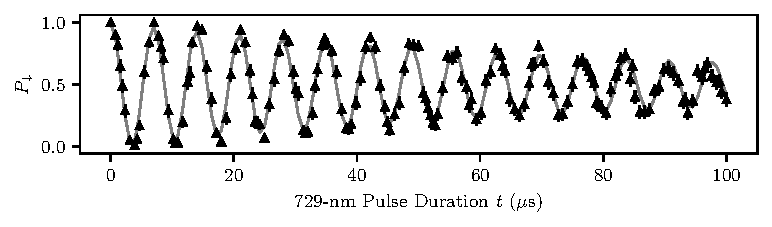
\includegraphics[width=\linewidth]{
            figures/pdf_figure/ch4/long_flop.pdf
            }
        \end{center}
        \caption{Rabi oscillations due to on-resonant 729-nm beam.  Estimated probability $P_\downarrow$ at each time step is an average of 200 individual experimental shots. The solid line is a fit using decaying oscillation model given by equation~\ref{eqn:decay_rabi}.
            }
        \label{fig:Long Flop}
    \end{figure}

    With the resonant frequency well calibrated, the pulse durations for various gates must be set. Here we outline the calibration routine for a $R_x(\frac{\pi}{2})$-gate, although this may be adapted for gate angles correspond to integer fractions of $2\pi$.\\
    We use a modified version of the RPE protocol to determine optimal gate durations. This protocol converges with a sufficiently close initial value for pulse duration $T_{\pi/2}$, and so a simple calibration using resonant Rabi oscillations is first described.\\
    The qubit is prepared in the computational eigenstate $\ket{\downarrow}$, followed by an on-resonant 729-nm carrier pulse inducing $R_x(\Omega t)$ rotations. The final state population is measured as a function of pulse duration to observe familiar Rabi oscillations. Figure~\ref{fig:Long Flop} displays these oscillations when using a global-addressing beam with a total power of $1~\unit{\milli\watt}$. Here each point corresponds to the average of 200 samples.
    The Rabi frequency, $\Omega$, and decay rate, $\lambda$, are determined through fitting the recovered populations to the model,
    \begin{equation}
        \label{eqn:decay_rabi}
        P_{\downarrow} = \frac{1 + e^{-\lambda t} \cos(\Omega t)}{2}.
    \end{equation}
    In this case, the Rabi frequency is found to be
    $\Omega = 2\pi\times 0.1433(1)$~\unit{\MHz}, and the decay rate $\lambda =
    0.0104(6)~\mu$s$^{-1}$.
    From this a first-guess pulse duration of $T_{\pi/2} \approx 1.75$~\unit{\us} can be
    estimated.
    This is a sufficient initial value to calibrate further, however
    it does not account for any amplitude ramps or dead-time of the optical-pulse compared to the digital control signal.\\
    RPE provides a higher-precision calibration, that may account for
    non-square-pulse profiles. The protocol is simply adapted from the RPE
    method described above by setting the initial base probe as a single
    $R_x(\frac{\pi}{2})$-pulse, with duration $t_0 = T_{\pi/2}$. The pulse is
    repeated $2^k$ times up to $k_\mathrm{max}$ (inferred from characteristic decay time $\tau
    = \frac{1}{\lambda}$) applications of the $R_x(\frac{\pi}{2})$-pulse. The phase angle in the $yz$-plane is determined through applying an additional $R_x(\theta_f)$ rotation with angle $\theta_f \in [0,\frac{\pi}{2},\pi,\frac{3\pi}{2}]$, before measurement. 
    The
    final base phase accumulated, $\theta_0$, is determined after applying the
    phase unwrapping protocol given above. Any deviation between this measured
    phase and the target, $\frac{\pi}{2}$, may be
    subsequently calibrated by rescaling the original pulse in time by factor $s
    = \frac{\pi}{2\theta_0}$.\\

    This method, along with the transition frequency calibrations given above,
    provide an efficient method to calibrate systematic offsets of single qubit
    rotation gates driven through on-resonant carrier excitation. Next we
    discuss randomised benchmarking, a characterisation technique that provides
    a measure of remaining incoherent and systematic errors for the calibrated
    gates.

\subsection{Single-Qubit Randomised Benchmarking}
\label{sec:standard_rb}


    \begin{figure}
        \begin{center}
        \noindent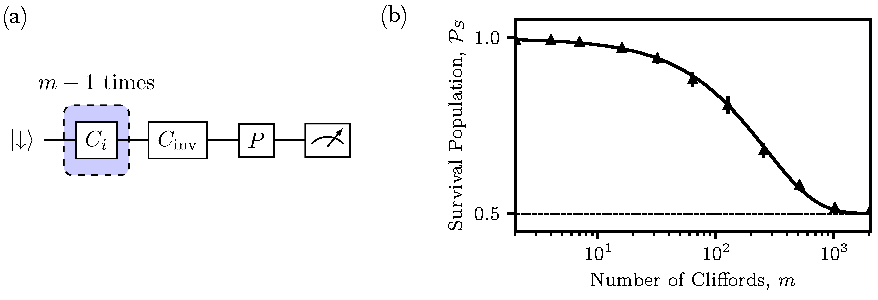
\includegraphics[width=\linewidth]{
            figures/pdf_figure/ch4/rb.pdf
            }
        \end{center}
        \caption{
            Standard randomised benchmarking applied to a single qubit. Panel a)
            shows the required circuit for a random sequence of Clifford gates,
            $C_i$, of total length $m-1$, with a final inverting Clifford,
            $C_\mathrm{inv}$, and a random Pauli gate, $P$, before measurement
            in the computational basis. Panel b) shows the survival probability,
            $\mathcal{P}_S$, versus Clifford sequence length, $m$.
            Each point is found by averaging over $r=50$ and $s=50$ repeats for each
            $m$. The solid line is a fit using the decay model given by
            equation~\ref{eq:RBM_decay}, the dashed line is the expected
            asymptote for a fully depolarised single qubit.
            }
        \label{fig:rbm}
    \end{figure}

    A further characterisation protocol is required to quantify the performance
    of single-qubit gates under both systematic and incoherent noise.
    A scalable class of methods, prevalent in quantum
    computation, is that of randomised benchmarking (RB). We will give a short
    description of RB here, but further details of the goals of
    characterisation, and complementary techniques to RB are discussed in
    chapter~\ref{ch:k-copy}~\S~\ref{sec:k-copy_char}.\\

    The purpose of RB is to simplify a general completely positive, trace preserving (CPTP) error channel by enforcing the
    symmetry of a chosen group on the channel~\cite{hashim_practical_2025}.
    The general error channel is described by the map acting on the space of density matrices,
    \begin{equation}
    \mathcal{E}(\hat\rho): \mathbb{C}^{d\times d}\rightarrow\mathbb{C}^{d\times d}
    \end{equation}
    where $d$ is the Hilbert space dimension.
    The symmetry is enforced on the channel through twirling --- averaging a channel $\mathcal{E}$
    over a group $\mathcal{G}$.
    A treatment of the action of twirling on a CPTP channel is given
    in~\S~\ref{app:twirling} in the context of \emph{k-copy}
    RB, an extension to standard RB methods for a single qubit~\cite{knill_randomized_2008}.\\
    The resulting simplified channel is
    then quantified to obtain metrics of the performance of the executed circuit.
    This protocol thus can reduce the problem to measuring $O(1)$
    parameters, rather than the $O(d^4)$ parameters required for a general
    quantum channel acting on a Hilbert space with dimension $d$. Furthermore, RB is
    particularly robust to state-preparation and measurement errors (SPAM),
    allowing for the isolation of errors originating from imperfect SPAM, to
    errors originating from the qubits idling or from the execution of gates.\\

    Practically RB protocols are simple to implement, approximating the twirling procedure to the generation
    and execution of an ensemble of
    random gate sequences of varying lengths,
    $m$. We focus on the ``standard'' RB sequence, enforcing the single-qubit
    Clifford group symmetry onto a single-qubit
    error channel~\cite{knill_randomized_2008}. The aim of standard RB is to twirl
    over the single-qubit unitary group, $SU(2)$, which takes the Haar measure,
    and transforms single-qubit error channels to highly-symmetric depolarising
    type channels, fully expressed by a single parameter, $\lambda$,
    \begin{equation}
    \mathcal{E}_{dp}(\hat\rho) = (1-2\lambda)\hat\rho + \lambda I_2 \mathrm{Tr}(\hat\rho),
    \end{equation}
    where $\mathcal{E}_{dp}$ is the resulting twirled channel, and $I_2$ is the $2\times 2$ identity matrix.
    Unfortunately, $SU(2)$ is continuous, as such it is impractical to average over the entire group.
    However, there are certain subgroups of $SU(2)$ that can be averaged over to
    recover an approximation of the Haar measure over $SU(2)$, up to the moment
    $t$. These subgroups are known as unitary $t$-designs of $SU(2)$.
    The single-qubit Clifford group, $Cl_1$, is a known 2-design, and consists of only 24 elements~\cite{dankert_exact_2009}.\\

    The standard RB implementation for one sequence is presented in Figure~\ref{fig:rbm}~(a), and the full sequence is as follows:
    \begin{enumerate}
        \item The qubit is initialised to $\ket{\downarrow}$. 
        \item A sequence of $m-1$ single qubit Clifford gates, $C_i$, are applied, with each gate randomly sampled from the Clifford gate-set. 
        \item A final ``inverting'' Clifford gate, $C_\mathrm{inv}$, is applied which is chosen such that the full Clifford gate sequence is equivalent to the identity operation.
        \item A random Pauli gate, $P\in\{I,X,Y,Z\}$, is applied
        with equal probabilities\footnote{This acts to randomise the final outcome between
        computational states $\ket{\downarrow}$ and $\ket{\uparrow}$, enforcing a further symmetry
        on any state-preparation and measurement error component.}.
        \item The population is measured in the computational basis, with shots resulting in the expected outcome (accounting for the random Pauli) labelled as survivals, $S$, and opposite outcomes labelled as failures, $F$.
        \item Steps 1-5 are repeated $s$ times to find the average survival population, $\mathcal{P}_S$.
        \item Steps 1-6 are repeated $r$ times with different random sequences for sequence with length $m$. 
        \item Steps 1-7 are repeated for a chosen set of sequence lengths, $m$, here log-sampling $m$ up to some $m_\mathrm{max}$.
        \item The average survival populations versus sequence length, $m$, are fit to a decay model to extract a depolarising error per Clifford gate, $\varepsilon_c$, and a SPAM error $\varepsilon_\mathrm{sp}$.
    \end{enumerate}
    The decay model used to find the fidelity versus number of Clifford gates is given by,
    \begin{equation}
    \label{eq:RBM_decay}
        \mathcal{P}_S(m) = \frac{(1 - 2 \varepsilon_\mathrm{sp}) (1 - 2\varepsilon_c)^m + 1}{2},
    \end{equation}
    where the first term in brackets is the probability of no error during SPAM, and the second, exponential term provides the probability of not depolarising during a sequence of length $m$.\\

    \begin{figure}
        \begin{center}
        \noindent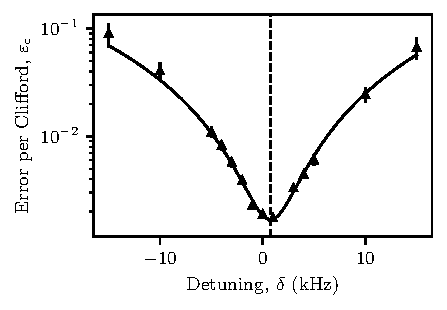
\includegraphics[width=0.5\linewidth]{
            figures/pdf_figure/ch4/rb_detuning.pdf
            }
        \end{center}
        \caption{
            Calibrating the relative detuning between the 729-nm laser and the
            qubit during the application of $\frac{\pi}{2}$-pulses. 
            Each point
            corresponds to the extracted error-per-Clifford from standard RB.
            The solid line is the fit of a quadratic model, the dashed line is
            the extracted center frequency.
            }
        \label{fig:rb_detuning}
    \end{figure}
    This scheme is applied experimentally to characterise the performance of the calibrated single-qubit gates.
    The 24 Clifford gates are decomposed into
    sequences of $R_x(\pm \frac{\pi}{2})$ and $R_x(\pm \frac{\pi}{2})$, with an average of 2.17 $\frac{\pi}{2}$-pulses per Clifford gate.
    Figure~\ref{fig:rbm}~(b) shows the average survival populations for a log-sampled range of sequence lengths up to $m_\mathrm{max} = 2048$ Clifford gates. Each point corresponds to an average over $r=50$ randomisations, and $s=50$ sample repeats per randomisation. The solid line follows equation~\ref{eq:RBM_decay}, with fit parameters, $\varepsilon_c=1.9(1)\times10^{-3}$, and $\varepsilon_\mathrm{sp}=3(1)\times10^{-3}$. The dashed line is the expected asymptote for a fully depolarised qubit. Error bars show the standard error of the average survivals for each random sequence for a given length $m$. From $\varepsilon_c$, we find a single $R_x(\frac{\pi}{2})$ average fidelity of $\mathcal{F}_{\pi/2}=1-\frac{\varepsilon_c}{2.17}=99.913(2)\%$.
    The measured SPAM is consistent with the independently characterised state preparation (\S~\ref{sec:Stateprep}) and measurement (\S~\ref{sec:Measurement}) errors of $\sim 10^{-3}$, and $\sim 10^{-4}$ respectively.\\

    We attribute the single-qubit rotation error to the finite-temperature of the radial modes. Expanding the light-matter interaction Hamiltonian given in equation~\ref{eqn:LD_regime} to second order in the Lamb-Dicke parameter, the carrier Rabi frequency is modulated depending on motional Fock state, $n$, as~\cite{leibfried_quantum_2003},
    \begin{equation}
    \Omega_n\approx \Omega\left(1-\eta^2\left(n+\frac{1}{2}\right)\right),
    \end{equation}
    where $\eta$ is the Lamb-Dicke parameter. For a thermal distribution each shot will result in a different rotation angle leading to a thermal dephasing error. For small rotation errors, the fidelity averaged over the Haar measure (see Appendix~\ref{sec:fidelity}) is given to first order by $\mathcal{F} =1-\frac{1}{3}\langle \theta^2\rangle$. If targetting an $R_x(\frac{\pi}{2})$-gate, the expected fidelity due to thermal errors is then,
    \begin{equation}
        \mathcal{F}_{\pi/2}(\bar{n})=1-\frac{1}{12}\pi^2\eta^4 (2\bar{n}^2 + \bar{n}).
    \end{equation}
    The radial modes for our target trapping frequencies ($\approx 2.5~\unit{\mega\hertz}$) have Lamb-Dicke parameters of $\eta\approx0.05$. For these experiments the radial modes are only Doppler cooled. In the following section on cooling,~\S~\ref{sec:Cooling}, we will determine the Doppler limit for these modes to be $\bar{n}_d \approx 4$. Using these two estimated parameters, we expect a fidelity due to thermal errors of $\mathrm{F}_{\pi/2,\mathrm{th}}=99.96\%$. This is similar in magnitude to the measured value and makes the assumption cooling is optimised to reach the Doppler limit. The single-qubit gate fidelity measured here is sufficient for the projects in this thesis, however if a lower error is required, we will be required to sub-Doppler cool all radial modes. \\

    RB can be used to calibrate systematic errors, however requiring many more samples than the RPE protocol described above. Figure~\ref{fig:rb_detuning} presents the detuning of the 729-nm laser with respect to the resonant frequency extracted by RPE. The points correspond to the extracted $\varepsilon_c$ from RB sequences with the same parameters as used for Figure~\ref{fig:rbm}~(b). The solid line is a quadratic fit, with center frequency $\delta=2\pi\times 0.76(8)~\unit{\kilo\hertz}$. The RPE protocol does not account for the Stark-shift due to the 729-nm beam, as such we see a frequency shift between the qubit and laser when probing by RB.\\
    We use standard RB as a daily characterisation experiment to verify consistent performance of the single-qubit gates. In chapter~\ref{ch:k-copy} we show further utility of single-qubit Clifford RB using a novel extension to parallel single-qubit Clifford application in a multi-qubit register.


\subsection{Spin Coherence Times}
\label{sec:Coherence}
% Main points:
    % Quote coherence times comparing:
        % Transitions with diff mag sensitivity
% Pre reqs:
    % Available transitions
    % 729 laser system
    \begin{figure}
        \begin{center}
        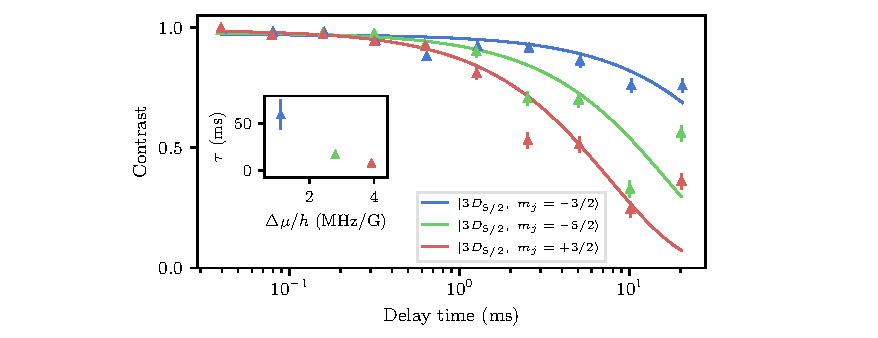
\includegraphics[width=\linewidth]{
            figures/pdf_figure/ch4/spin_coherence.pdf
            }
        \end{center}
        \caption{
        Coherence times of three quadrupole transitions with varying magnetic
        field sensitivities. Points correspond to the extracted contrasts of
        Ramsey fringes. Solid lines are exponential fits to determine the
        $\frac{1}{e}$ coherence time, $\tau$. The inset plot shows the measured
        coherence time as a function of the magnetic field sensitivity,
        $\Delta\mu/h$, of the transition being probed.
            }
        \label{fig:coherence_times}
    \end{figure}

    Qubit decoherence may originate from uncontrolled fluctuations of the qubit transition frequency or from phase noise on the laser driving the qubit transition. Decoherence directly contributes to loss of fidelity of qubit operations, and will limit the circuit-depths possible on our apparatus.\\
    Both electric and magnetic field noise can lead to qubit transition frequency fluctuations.
    The quadrupole transitions between the ground state $\ket{4S_{1/2}, m_j=-1/2}$ and the metastable manifold $\ket{3D_{5/2}}$ in \ca are first order sensitive to any external magnetic fields. As such, even with the MuMetal magnetic shield in place, external magnetic fields are expected to be the dominant noise source. To verify this, and benchmark the current decoherence time, the Ramsey contrast is measured as a function of delay duration. 
    The Ramsey sequence is as follows:
    \begin{enumerate}
        \item Prepare the qubit in $\ket{\downarrow}$. 
        \item A $R_y(\pi/2)$-pulse is applied. preparing the state $\ket{+} = \frac{1}{\sqrt{2}}(\ket{\downarrow} + \ket{\uparrow})$.
        \item The system is left to evolve for Ramsey delay, $t_{\rm RAM}$.
        \item A variable $R_\phi(\pi/2)$-pulse is applied.
        \item The population of $\ket{\downarrow}$ is measured.
        \item Repeat steps 1-5 for different values of $\phi$ to find the contrast of the Ramsey fringe.
        \item Repeat steps 1-6 for different values of $t_{\rm RAM}$ to find the decay in contrast with time. 
    \end{enumerate}

    This Ramsey fringe contrast is directly proportional to the coherence of the resulting noisy state, $\hat\rho$, given by matrix element, $\rho_{\da,\ua}$. \\
    Figure~\ref{fig:coherence_times} shows the coherence time of
    three quadrupole transitions:\\
    $\ket{4S_{1/2},~m_j=-1/2} \leftrightarrow \ket{3D_{5/2},~m_j=\lbrace -5/2,
    -3/2, +3/2\rbrace }$. These transitions have magnetic field
    sensitivities of $\Delta\mu/h = \{2.799, 1.119,
    3.922\}~\unit{\MHz\per\gauss}$ respectively (calculated using equation~\ref{eqn:mag_sens}). The contrast decays for all
    three qubits are shown in the figure. 
    The $\frac{1}{e}$-coherence time is extracted by fitting exponential decays
    to the contrasts. Generally, exponential decays indicate the timescale of
    the noise is fast compared to the Ramsey probe durations, whilst Gaussian
    decays indicates comparatively slow drifts. Neither exponential nor Gaussian
    well describe the measured decays here due to the strong
    periodic structure above the exponential decay. This suggests a strong
    narrow-band coherent component to the noise. At the time scale of $\approx
    20~\unit{\milli\second}$ we expect to see the effects of UK mains hum, which
    likely cause this structure. Regardless, fitting the exponential envelope
    suggests a coherence time of $17(4)~\unit{\milli\second}$ for the qubit
    transition, $\ket{4S_{1/2},~m_j=-1/2} \leftrightarrow
    \ket{3D_{5/2},~m_j= -5/2}$.
    The inset plot shows the extracted coherence time as a function of transition magnetic field sensitivity. There is a clear dependency between the coherence time and the magnetic field sensitivity,
    suggesting that magnetic noise is dominant.\\

\subsection{Single-ion Addressing}
\label{sec:Single Addressing char}
    \begin{figure}
        \begin{center}
        \noindent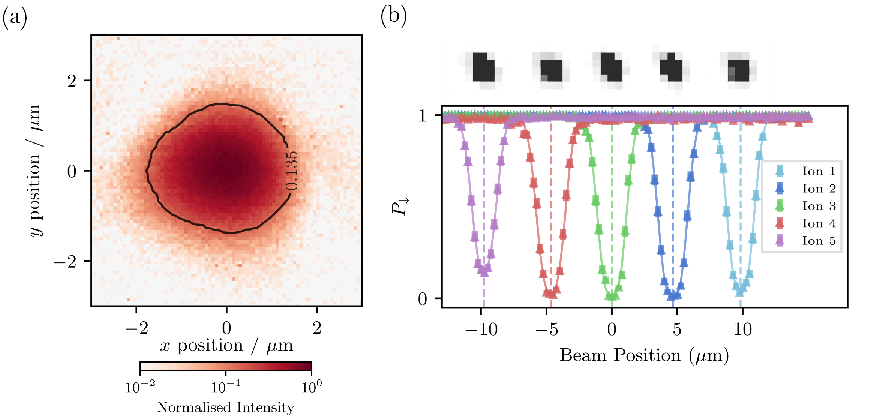
\includegraphics[width=\linewidth]{
            figures/pdf_figure/ch4/sa.pdf
            }
        \end{center}
        \caption{
            Characterisation of the single-ion addressing system using the ion as a probe. a) The normalised intensity of the 
            focussed 729-nm beam at the ion-plane. The $1/e^2$-waist is highlighted by the contour. b) Demonstration of spatial selective addressing by scanning the beam across a 5-ion chain while applying $R_x(\pi)$-gates calibrated for ion 3. The probability of observing $\ket{\downarrow}$, $P_\downarrow$ is shown for each ion.
            }
        \label{fig:sa_char}
    \end{figure}

The single-ion addressing system, introduced in~\S~\ref{sec:Single Addressing
System}, is calibrated and characterised using the ion as a sensor. We verify
that the beam waist at the ion plane approximately matches the designed
specification, and we measure the crosstalk due to an addressed neighbouring
ion. Crosstalk can cause structured coherent errors acting on the qubit
register, which can have particularly adverse effects to error correction and
mitigation protocols that assume independent, uncorrelated noise on each qubit.
As such, designing an addressing system for low-crosstalk, and verifying its
performance is critical.
\\

The intensity profile of the beam in the ion plane is measured by Rabi
oscillations on a single-trapped ion while scanning the beam position in a 2D
grid. To efficiently measure this 2D array, a fixed Rabi pulse duration is used,
although we note that similar measurements can be made with adaptive pulse
durations, or through using RPE type protocols to improve the sensitivity of
these measurement. To avoid ambiguity of the accumulated phase, we ensure that
at the point of maximum field amplitude the accumulated phase does not wrap,
$\theta_\mathrm{max} < \pi$.
The relative optical intensity may then be extracted by considering
equation~\ref{eqn:decay_rabi}, assuming a negligible decay rate, $\lambda$, and
recalling that $\Omega\propto\sqrt{I}$, yielding,
\begin{equation}
    \frac{I(x,y)}{I_\mathrm{max}} = \left(\frac{\mathrm{acos}\left(\sqrt{P_\downarrow(x,y)}\right)}{\theta_\mathrm{max}}\right)^2.
\end{equation}
The normalised intensity profile extracted by this method is shown in
Figure~\ref{fig:sa_char}~(a). The qubit is initialised in $\ket{\downarrow}$
using the global addressing beam, and the total single-addressing beam power is
stabilised to $20~\unit{\micro\watt}$. The black contour signifies the
$\frac{1}{e^2}$
waist. The spot closely resembles the expected Gaussian shape, with some
aberrations, especially leading to a shoulder in the $-x$ direction. Fitting a
2D Gaussian distribution, we find $\frac{1}{e^2}$-waists of
$\omega_x=1.584(3)~\unit{\micro\meter}$, and
$\omega_y=1.386(2)~\unit{\micro\meter}$. These closely match the target waist of $1.5~\unit{\micro\meter}$.\\
The crosstalk is measured by scanning a single beam across a 5-ion chain. The
axial frequency of the trap is set to $0.7~\unit{\mega\hertz}$, to provide an
ion spacing of $\approx 5\unit{\micro\meter}$. When addressing the central ion
of the chain, ion 3, we may observe Rabi oscillations on all qubits
simultaneously to extract the relative Rabi frequency crosstalk. The Rabi
frequency is determined through fitting equation~\ref{eqn:decay_rabi}, finding
frequencies of $2\pi\times\{1.0(1), 1.67(5), 281.7(5), 7.96(1),
5.29(1)\}~\unit{\kilo\hertz}$ for ions 1 to 5 respectively. This corresponds to
intensity crosstalks of $\{0.12(4), 0.35(2),-,7.99(3),3.53(1)\}\times10^{-4}$ respectively.\\
To highlight this spatial selectivity, we show the beam scanning across the 5-ion chain with a fixed pulse duration.
For reference, above this plot we show fluorescence of the 5-ion chain as viewed by the imaging camera. 
The fixed Rabi-pulse duration is calibrated to be a $R_x(\pi)$-pulse when acting
on the central ion. Figure~\ref{fig:sa_char}~(b) shows the measured populations,
$P_\downarrow$, as a function of beam position along the axial ion-chain
direction. The points correspond to populations averaged over $200$ samples,
with the population for each ion gathered simultaneously using the spatially
resolved readout, as discussed in~\S~\ref{sec:Measurement}. The solid lines
follow the simple model inferred from the expected Gaussian waist of the beams, 
\begin{equation}
P_{\downarrow,i} = 1 - \sin\left(A_i\mathrm{exp}\left(\frac{-(x - x_i)^2} {\omega^2}\right)\right)^ 2,
\end{equation}
where $x_i$ is the central position for ion, $i$, and $A_i$ is included to account for a drop in field amplitude due to any
misalignment between the addressing axis and the ion-chain, or due to changes in
diffraction efficiency of the AODs when driving them at different frequencies.
Practically we may calibrate the beam power set-point to balance any
Rabi-frequencies for every addressing configuration to mitigate these small
misalignments and limited bandwidths of the AODs.\\

The achieved waist of $\approx 1.5~\unit{\micro\meter}$ allows for high
intensity fields at the qubits, exemplified here by the low
$20~\unit{\micro\watt}$ 729-nm beam power required for driving $\approx
1~\unit{\micro\second}$ $R_x(\frac{\pi}{2})$ gates. The low intensity crosstalk
of $<10^{-3}$ for neighbouring ions is sufficient for the projects demonstrated
in this thesis. If lower crosstalk errors are required, it is likely this may be
reduced to $<10^{-4}$ solely through further optimisation of beam alignment
through the optical train. This is suggested by the current asymmetry of
crosstalk errors either side of the addressed qubit. Furthermore, as the
crosstalk error is coherent, it may be further suppressed using composite pulse
sequences~\cite{fang_crosstalk_2022}.

\section{Motion}
\label{sec:Motion}
% Main points:
    % Quote characterisation method and values for various motional measurements.
    % Highlight where we are not yet at the capability we need.
    % State what improvements we plan to add.
% Pre reqs:
    % Motivation for control of motion of ion
    % Trap RF DC
    % Laser systems

    We outline methods to track the mode frequencies, cool the motion of the
    qubit, quantify thermal heating of the motion, and characterise the qumode
    coherence time. These methods are necessary for control over qumodes for
    information, or for using the common motion as a means to entangle two
    qubits.\\

    Motion of ions trapped in the same potential can be described by a set of
    normal modes~\cite{james_quantum_1998}. These modes are labelled with respect
    to the ion chain geometry: axial modes oscillate parallel with the chain,
    and radial modes oscillate perpendicular to the chain. Due to the geometry
    of the 729-nm beam access with respect to the ion chain (see
~\S~\ref{sec:Vacuum System}), only the radial modes can be addressed in
    our system. For the \emph{NPL} trap (see~\S~\ref{sec:The Ion Trap}),
    the radial modes frequencies are non-degenerate. In our system, for a single
    ion, the mode frequencies are approximately $\omega_{\rm upper}
    =2\pi\times2.9$~\unit{\MHz}, $\omega_{\rm lower} = 2\pi\times2.0$~\unit{\MHz},
    and 
    $\omega_{\rm axial} = 2\pi\times1.0$~\unit{\MHz}, where ``upper'' and ``lower''
    are the two radial modes. All
    results in the following section are using
    the upper radial mode. \\


\begin{figure}
    \begin{center}
    \noindent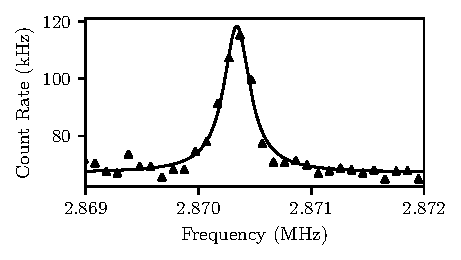
\includegraphics[width=0.5\linewidth]{
        figures/pdf_figure/ch4/tickle.pdf
        }
    \end{center}
    \caption{
        Motional mode resonance measured by RF ``tickle'' experiment. Points correspond to fluorescence rate measured by the camera while the solid line is a Lorentzian model fit.
        }
    \label{fig:tickle}
\end{figure}
\subsection{Calibrating Mode Frequencies}
\label{sec:tickle}
    The radial mode frequencies are proportional to the RF voltage (equation~\ref{eqn:pseudo_pot}), as such any amplitude drift on the RF chain translates to mode frequency drift. The efficiency of the resonator, as discussed in~\S~\ref{sec:Trap RF Chain}, is dependent on ambient temperature, and is currently not actively stabilised. As such the mode frequencies are routinely (order minutes) measured to track and update the frequency set point for interactions involving the mode.\\
    The motional mode frequency is measured via an RF ``tickle'' experiment.
    This consists of short ($\approx 1~\unit{\milli\second}$) RF field pulses applied to one
    of the trap DC electrodes which has a non-zero electric field projection to
    the mode we wish to probe. The frequency of the RF field is scanned around
    the expected motional mode frequency, and when resonant drives the motion
    of the ion. Excess motional amplitude is measured by observing an increase in
    fluorescence when driving a closed dipole transition detuned to a nonlinear
    region of the resonance. The motional induced sidebands at this nonlinear
    point are unbalanced leading to a modulation of fluorescence. Here the
    397-nm laser is set to provide approximately 1 saturation intensity of light
    to avoid power broadening the dipole transition. The 397-nm is red-detuned
    100~\unit{\MHz} from resonance.  The 866-nm is set to typical readout parameters to
    repump any population trapped in the $D$-manifold. The modulated
    fluorescence is integrated over $\approx 1~\unit{\milli\second}$ leading to
    an increased average count rate when the RF tone is resonant with the mode
    frequency.\\
    Figure~\ref{fig:tickle} shows the typical fluorescence count rate for this mode frequency calibration scan on the upper radial mode. A Lorentzian profile is fit to extract central mode frequency $\omega_\mathrm{upper}=2\pi\times2.87034(2)~\unit{\mega\hertz}$, and FWHM of $280(50)~\unit{\hertz}$. The uncertainties of these parameters are determined by the bootstrapping method using $1000$ re-samplings.

\subsection{Cooling}
\label{sec:Cooling}
% Main points:
    % Introduce why we want to cool
    % Doppler cooling
    % Sideband cooling
% Pre reqs:
    % Motional mode and beam geometry
    % Laser systems 
    % Trapping

    For any interaction that involves the motion of the ion, it is essential to
    both prepare and measure the motional state with high fidelity. For all
    motional interactions considered in this thesis, the ion is initially
    prepared as close as possible to the motional ground state, with a mean
    phonon number $\bar{n} \approx 0$. This is done by an initial stage of
    Doppler cooling, followed by pulsed sideband cooling on the 729-nm
    transition. The final motional state is characterised by measuring the
    population in Fock states using RSB and effective BSB pulses.\\

\subsubsection{Doppler Cooling}
% Main points:
    % Quote final temperature reached (theory?)
    % Describe cooling parameters
% Pre reqs:
    % Motional mode and beam geometry
    % Laser systems 

    Doppler cooling relies on light incident on a moving ion 
    appearing frequency shifted in the ion's rest frame. For Doppler cooling
    of \ca, both the 397-nm and 866-nm lasers are applied. The 397-nm laser is red-detuned from the dipole $\ket{4S_{1/2}}\leftrightarrow\ket{4P_{1/2}}$ transition, leading to preferential
    scattering of 397-nm photons that have a net cooling effect~\cite{wineland_laser_1979}. The excited $4P_{1/2}$ level decays via two channels: emission of a 397-nm photon back to $\ket{4S_{1/2}}$, or an 866-nm photon to $\ket{3D_{3/2}}$, with a branching
    ratio of 14.5~\cite{ramm_precision_2013}. Since many photon scattering events are required, the cooling cycle must be closed. To prevent population trapping in the metastable $\ket{3D_{3/2}}$ level, the 866-nm laser is applied on resonance during cooling.\\
    Equilibrium
    is reached when the cooling rate balances
    photon recoil heating. Assuming the 397-nm transition is broadened only by its natural linewidth $\gamma$, 
    the minimum Doppler temperature is,
    \begin{equation}
    T_{\rm Doppler} \approx \frac{\hbar\gamma}{2k_B},
    \end{equation}
    where $\hbar$ is the reduced Planck constant, and $k_B$ is Boltzmann's constant~\cite{wineland_laser_1979}.\\
     For
    $^{40}$Ca$^+$, the natural linewidth of the 397-nm transition is $\frac{\gamma}{2\pi} =
    21$~\unit{\MHz}\cite{morton_atomic_2003}, giving $T_{\rm Doppler} = 0.5$~\unit{\milli\kelvin}. 
    Given a mode frequency, the expected mean phonon number is,
    \begin{equation}
        \bar{n} = \frac{1}{e^{\hbar\omega/k_B T}-1}.
    \end{equation}
    For a radial mode with frequency $\omega \approx 2\pi\times2.5$~\unit{\MHz}, the Doppler limit is approximately
    $\bar{n} \approx 4$. 
    The parameters used here for Doppler cooling are summarised in Table~\ref{tab:397_parameters}. \\

\subsubsection{Sideband Cooling}
% Main points:
    % Quote final temperature reached
    % Describe SBC pulse sequence
    % We use a closed transition
% Pre reqs:
    % Motional mode spectra
    % Laser systems 
    % Rabi flopping

    \begin{figure}
        \begin{center}
        \noindent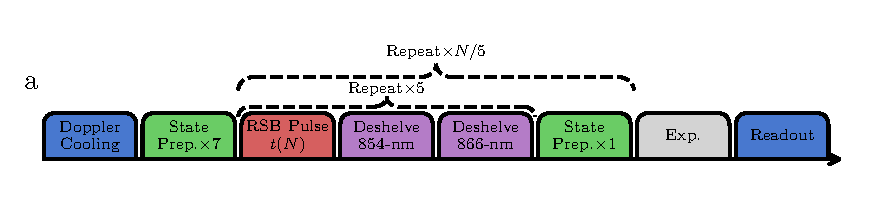
\includegraphics[width=\linewidth]{
            figures/pdf_figure/ch4/pulse_sequence.pdf
            }
        \noindent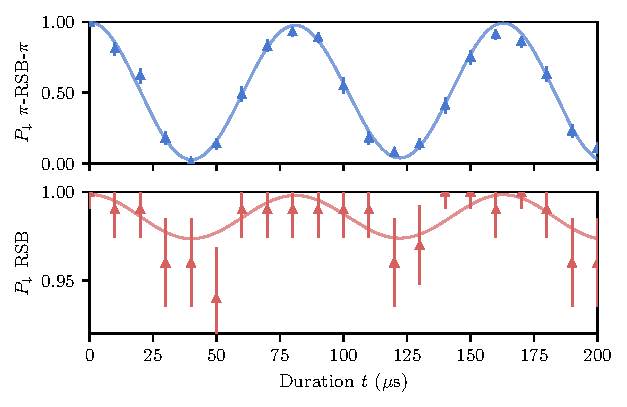
\includegraphics[width=0.75\linewidth]{
            figures/pdf_figure/ch4/sideband_thermometry.pdf
            }

        \end{center}
        \caption{
            (a) Example pulse sequence for one experimental shot including pulsed sideband cooling. The \emph{Exp.} block represents an arbitrary sequence of operations, for the experiment under study, such as a thermometry sequence.
            The blue blocks represent Doppler cooling and readout
            (\S~\ref{sec:Measurement}), the green blocks represent qubit
            state preparation (\S~\ref{sec:Stateprep}), the red blocks are
            RSB pulses with varying durations $t(N)$, and the purple blocks are
            deshelving pulses. After every 5 sideband cooling pulses, there is
            an interleaved state preparation sequence to ensure there is no
            population trapped outside of the closed cooling cycle. The RSB
            length is linearly increased with pulse number $N$, up to the
            expected RSB $R(\pi)$-pulse duration for $n=1$.  
            (b, c) Thermometry scans after Doppler and sideband cooling.
            The red points are the populations measured via on-resonance RSB
            pulses, and the blue points are the populations after a sequence of
            $R(\pi)$-RSB-$R(\pi)$ with varying RSB probe durations. The solid
            lines are fits to a thermal Fock state distribution, with truncation
            at $n = 100$. The extracted mean occupation number is $\bar{n} =
            0.03(1)$, and $\eta\Omega/(2\pi) = 11.6(1)$~\unit{\kHz}. 
            }
        \label{fig:SBC}
    \end{figure}
    \begin{table}
        \begin{center}
        \begin{tabular}{|c|l|}
            \hline
            Parameter & Value \\
            \hline
            729-nm laser power & 3.0~\unit{\mW}\\
            729-nm laser detuning & -4.0~\unit{\MHz}*\\
            729-nm pulse duration $N = 1$ & 2.5~\unit{\us}\\
            729-nm pulse duration $N = N_{\rm max}$ & 33~\unit{\us}  \\
            Repumping 866-nm duration & 14~\unit{\us}\\
            Deshelving 854-nm duration & 5~\unit{\us}\\
            Number of cooling cycles $N_{\rm max}$ & 50\\
            \hline
        \end{tabular}
        \end{center}
        \caption{
            *729-nm detuning is relative to the $\ket{4S_{1/2},~m_j=-1/2} \leftrightarrow \ket{3D_{5/2},~m_j=-5/2}$ transition frequency.\\
            Experimental parameters used for sideband cooling. Other parameters for the repump and deshelve pulses are the same as for state preparation, see Table~\ref{tab:state_prep_parameters}. The 729-nm laser is detuned to the RSB resonance for the upper radial mode, $\omega_{\rm upper}/2\pi = 4.0$~\unit{\MHz}, and the pulse duration for $N=N_{\rm max}$ is chosen to be the expected RSB $R(\pi)$-pulse duration for $n=1$. 
            }
        \label{tab:sbc_parameters}
    \end{table}

    To further cool the ions toward their motional ground state, resolved
    sideband cooling is used~\cite{diedrich_laser_1989}. As discussed in~\S~\ref{sec:Motional Coupling}, red and blue sidebands (RSB and BSB) of the quadrupole transition are accessible, which may both flip the spin and add or remove a single phonon from the motional mode. For the $\ket{4S_{1/2}} \leftrightarrow
    \ket{3D_{5/2}}$ transition, at appropriate motional mode
    frequencies, interaction strengths, and using a narrow linewidth laser (\S~\ref{sec:Narrow Linewidth 729 Laser}), these sidebands can be resolved spectroscopically. The pulsed
    sideband technique employed consists of RSB pulses on the 729-nm transition, followed by
    deshelving, and repumping pulses on the 854-nm and 866-nm transitions
    respectively. 
    For efficient cooling, initial short 729-nm pulses are applied to preferentially excite the thermal population with high phonon number, as the pulse duration for RSB $R(\pi)$ is proportional to $\sqrt{n}$, where $n$ is the phonon number.  The RSB pulse length is linearly increased to the expected RSB $R(\pi)$-pulse duration for $n=1$.\\
    An example pulse sequence for a single experimental shot using sideband cooling, can be seen in
    Figure~\ref{fig:SBC} (a). Experimental parameters used are summarised in Table~\ref{tab:sbc_parameters}.\\
    We use the RSB of the quadrupole transition $\ket{4S_{1/2},~m_j = -1/2} \leftrightarrow \ket{3D_{5/2},~m_j = -5/2}$ as the subsequent deshelve and spontaneous decay from $\ket{4P_{3/2},~m_j=-3/2}$ to $\ket{4S_{1/2},~m_j=-1/2}$ forms a closed cycle, lessening the need for state-preparation pulses throughout the sideband-cooling sequence.\\

    To verify the efficacy of our sideband cooling, thermometry
    experiments are performed by probing Fock state populations. This is done using on resonance RSB pulses and effective BSB pulses composed of a $R_x(\pi)$-RSB-$R_x(\pi)$ pulse
    sequences. The spin population dynamics are measured as RSB
    pulse length, $t$, is varied. In the case of Fock state $\ket{0}$, there should be full contrast 
    ``BSB'' oscillations, and no visible oscillations when probed with RSB pulses. A thermal
    Fock state distribution~\cite{meekhof_generation_1996} (with truncation at Fock state = 100) is fitted to these
    signals to extract the mean occupation number, and $\eta\Omega$, the carrier
    Rabi frequency multiplied by the Lamb-Dicke parameter. A typical thermometry
    scan after Doppler and sideband cooling can be seen in
    Figure~\ref{fig:SBC} (b, c), where (b) shows the population after effective BSB pulses, and (c) shows the population after RSB$(t)$ pulses with duration $t$. The mean occupation
    number after sideband cooling is found to be $\bar{n} = 0.03(1)$, and $\eta\Omega =
    11.6(1)$~\unit{\kHz}.\\

\subsection{Heating Rates}
\label{sec:Heating}
% Main points:
    % Quote motional heating rates for mode we use (have access to).
    % Describe heating model?
% Pre reqs:
    % Thermometry
    % Motional modes
    % Trap

    \begin{figure}
        \begin{center}
        \noindent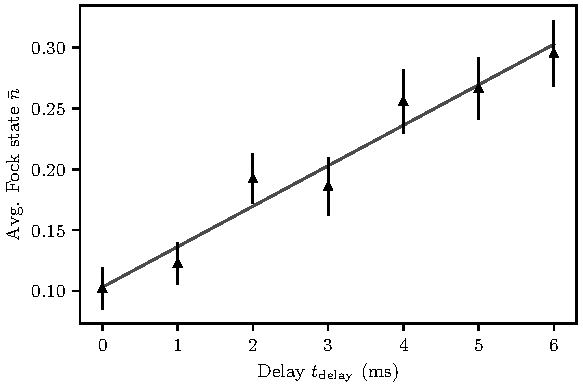
\includegraphics[width=0.667\linewidth]{
            figures/pdf_figure/ch4/heating_rate.pdf
            }
        \end{center}
        \caption{
            Heating rates of upper radial mode, measured by varying the delay between cooling and thermometry pulses. The solid line is a linear fit to the data, with slope $33(3)$~quanta/s. The error bars are given by the standard deviation of the fitted $\bar{n}$.
            }
        \label{fig:heating rates}
    \end{figure}

    After cooling the motion, the ion will return to a temperature in
    equilibrium with the environment. However, this process can be slowed by
    adequate isolation of the ion. In UHV ion trap systems (see~\S~\ref{sec:Vacuum System}), motional heating is predominantly caused
    by electric field noise from the ion trap~\cite{wineland_experimental_1998}.
    Noise due to thermal charge fluctuations at the trap surface can be 
    mitigated by increasing ion-electrode distances. The \emph{NPL} trap
    (\S~\ref{sec:The Ion Trap}), used here, has an ion-electrode 
    distance of 250~\unit{\um}, larger than most surface traps, but less than that of a
    macroscopic blade or rod style trap~\cite{milne_construction_nodate}.
    Heating rates were probed by a series of thermometry experiments, explained
    above, with varying delay
    times, $t_{\rm delay}$, between cooling and thermometry pulses. A typical plot can be seen in
    Figure~\ref{fig:heating rates}. The heating rate of the system
    was found by a linear fit, shown by the solid line, to be $33(3)$~quanta
    per second on the upper radial with mode frequency $\omega_\mathrm{upper} \approx 3~\unit{\MHz}$ on
    one ion. As will be discussed in~\S~\ref{sec:Motional Coherence}, the heating rate sets a limit for the motional coherence time.\\

% \subsection{Motional Mode Stability}
% \label{sec:Motional Mode Stability}
% \todo{Requires plot and main text numbers update, but we dont yet have data... 2025/11/07\\}
% % Main points:
%     % Quote motional mode drift 
%     % Explain why it is currently drifty
%     % Outline how this will be improved with the squareatron
% % Pre reqs:
%     % Trap

%     \begin{figure}
%         \begin{center}
%         \noindent\includegraphics[width=\linewidth]{
%             figures/pdf_figure/ch4/mode_drift.pdf
%             }
%         \end{center}
%         \caption{
%             \textbf{a)} Motional mode frequency drift over time. The radial motional mode frequency is measured by exciting motion using an RF field in resonance with the motional frequency, and looking at increased fluorescence. The resulting frequency trace is shown in blue. The green line shows a low pass filter of the data, with cut-off frequency of 1.67~\unit{\mHz}, corresponding to an assumed 10 minutes slow thermal drift. The motional mode frequency is typically calibrated every 10 minutes, which is indicated by the red line. 
%             \textbf{b)} Residuals from the measured data and expected calibrated mode frequencies. The standard deviation of these residuals suggests the typical mis-set detuning of the mode frequency in current experiments with automated mode frequency calibrations every 10 minutes.
%             \textbf{c)} Residuals from the measured data and the low passed trace. The standard deviation of these residuals are due to noise with period less than 10 minutes. 
%             }
%         \label{fig:mode drift}
%     \end{figure}

%     Due to thermal drifts and microphonics introducing amplitude and frequency
%     noise on the RF chain, drifts of the radial motional mode frequencies are
%     seen over time. As will be discussed in the following
%     section~\ref{sec:Motional Coherence}, this can lead to dephasing of the
%     motional state. Here, the current motional mode stability is characterised
%     to estimate its contribution to dephasing, and to set a benchmark for future
%     stability improvements. \\
%     To measure mode frequency drift, this sequence is repeated every 10 seconds
%     over multiple hours. A typical plot can be seen in figure~\ref{fig:mode
%     drift} $a$. Over this two hour period, the frequency had an absolute drift
%     of 1.5~\unit{\kHz}. Typically, we calibrate the mode frequency every 10
%     minutes, which is indicated with the red dashed line. Residuals between this
%     calibrated line and the data, shown in $b$, have a standard deviation of
%     $\sigma/(2\pi) = 203(8)$~\unit{\Hz}, giving the expected uncertainty of the
%     mode frequency detuning given our current periodic calibration routine. A
%     slow drift with frequency cut-off of 1.67~\unit{\mHz} is also fitted to the
%     data, shown in green. The residuals from this fit, shown in $c$, have a
%     standard deviation of $\sigma/(2\pi) = 94(4)$~\unit{\Hz}. This suggests that
%     the motional mode frequency is relatively stable over time scales shorter
%     than 10 minutes, but has a slow drift on longer time scales, which is likely
%     due to thermal fluctuations. \\
    
    % Tracking noise source
    % Show resonator scan
    % Explain we sit either on peak or edge
    % show mode drift of +- edge of resonator.
    % This suggests amplitude drift
    % XXX However, we can distinguish between amplitude or resonator frequency drifts by changing the trap RF frequency. Figure~\ref{fig: mode drift} shows the motional mode frequency versus the trap RF frequency. The quadratic responce seen is due to the bandwidth of the resonator. By probing two points If the central frequency of the resonator drifts over time
    

\subsection{Motional Coherence Times}
\label{sec:Motional Coherence}
% Main points:
    % Quote measured result for motional coherence time
    % Give estimate for what times we need for future experiments
    % Give estimate contributions from motional heating and from mode instability
    % What fix will we do for improving this - squareatron from prev section, resonator.
% Pre reqs:
    % Trap RF
    % Trap Resonator
    % Motional mode stability
    % SBC
\begin{figure}
    \begin{center}
    \noindent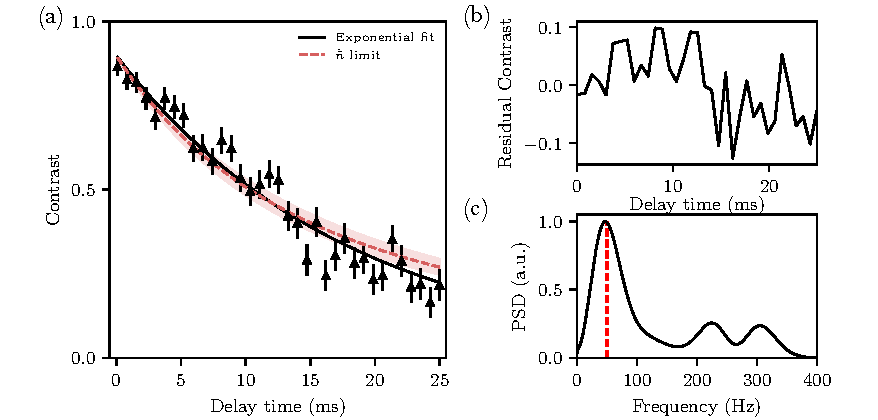
\includegraphics[width=\linewidth]{
        figures/pdf_figure/ch4/motional_coherence.pdf
        }
    \end{center}
    \caption{
        a) Motional coherence time measured by Ramsey interferometry using Fock
        states $\ket{0}$ and $\ket{1}$. Points are populations measured in
        $\ket{\downarrow}$ after the Ramsey sequence with varying delay time.
        The black dashed line is an exponential decay fit, with $\frac{1}{e}$
        coherence time $\tau = 18.0(8)$~\unit{\ms}, and initial contrast $C_0 =
        0.90(2)$. The red line corresponds to the expected decay due to the
        independently measured heating rate of $\dot{\bar{n}}=33(3)$~q/s. b)~Displays 
        the residual oscillations after subtracting the expected
        heating-rate profile. c)~Displays the PSD of the residual oscillations,
        with the dashed red line signifying $50~\unit{\hertz}$.
        }
    \label{fig:motional_coherence}
\end{figure}

    For both hybrid computation, and for two-qubit entangling gates via
    geometric phase gates, we require motional modes with long coherence times
    compared to the desired circuit length. Electric field noise on the trap RF,
    or fluctuating external fields cause decoherence of the qumode. The field
    noise can cause coherent errors, motional frequency dephasing, or thermal heating of
    the mode, depending on its coherence and underling frequency spectrum.
    Here the coherence time is quantified
    using Fock state interferometry --- a Ramsey technique with initial superposition states $\ket{\psi_{0m}}=(\ket{\downarrow, 0}+\ket{\downarrow, m})/\sqrt{2}$, where $m$ is a pure Fock state~\cite{turchette_decoherence_2000}. The acquired Ramsey phase is mapped to the optical qubit through sideband pulses. Fock state interferometry is
    easy to implement through driving resonant carrier and RSB gates, and is sensitive to both dephasing
    and mode-heating noise. We note that similar interferometry
    techniques based on cat states~\cite{monroe_schrodinger_1996} also 
    quantify decoherence, however with different
    sensitivities to both dephasing and heating. \\
    The Ramsey contrast decays is measured by the following sequence:
    \begin{enumerate}
    \item Prepare the ground state of both qubit and qumode, $\ket{\downarrow, 0}$. The qubit is first prepared via optical pumping, and the qumode is subsequently prepared by Doppler and resolved sideband cooling.
    \item A $R_y(\pi/2)$-pulse is applied on the carrier transition, preparing the state $(\ket{\downarrow, 0} + \ket{\uparrow, 0})/\sqrt{2}$.
    \item A RSB $R_\mathrm{RSB}(\pi)$-pulse is applied, preparing the state $\ket{\psi_{0m}}=(\ket{\downarrow, 0} + \ket{\downarrow, 1})/\sqrt{2}$.
    \item The system is left to evolve for Ramsey delay, $t_{\rm RAM}$.
    \item A RSB $R_\mathrm{RSB}(\pi)$-pulse is applied to map accumulated phase onto the qubit state.
    \item A variable carrier $R_\phi(\pi/2)$-pulse is applied.
    \item The population of $\ket{\downarrow}$ is measured.
    \item Repeat steps 1-7 for different values of $\phi$ to find the contrast of the Ramsey fringe.
    \item Repeat steps 1-8 for different values of $t_{\rm RAM}$ to find the decay in contrast with time.
    \end{enumerate}

    Figure~\ref{fig:motional_coherence}~(a) shows the recovered coherence contrast
    for variable Ramsey delays for the upper radial mode of a single ion, with
    frequency $\omega_\mathrm{upper}\approx 2\pi\times2.9~\unit{\mega\hertz}$.
    The black solid line indicates an exponential decay with a fit $\frac{1}{e}$ coherence time
    of $\tau = 18.0(8)$~\unit{\ms}, and initial contrast $C_0 = 0.90(2)$. The
    low initial contrast is attributed to imperfect RSB pulses due to a
    combination of finite residual mode temperature (expected around
    $\bar{n}=0.03$), and imperfect calibration of the sideband frequency and
    $\pi$-gate duration.
    The exponential, rather than Gaussian, profile of the decay suggests that the dominating noise
    source is correlated for durations much shorter
    than the Ramsey delay times~\cite{omalley_qubit_2015}. \\
    If motional-mode heating is dominant, the expected decay in the coherence 
    between Fock states $\ket{0}$ and $\ket{m}$ for an equal superposition is given by~\cite{turchette_decoherence_2000, kienzler_quantum_2015},
    \begin{equation}
        \rho_{0m}(t)=\frac{1}{2(1+\dot{\bar{n}}t)^{m+1}},
    \end{equation}
    where $\rho_{0m}$ is the off-diagonal density matrix element, and 
    $\dot{\bar{n}}$ is the heating rate in phonons per second.
    Taking $m=1$, and using the above protocol mapping the motional coherence to the spin-qubit, we find spin populations,
    \begin{equation}
    P_\da(t) = \rho_{01}(t) + \rho_{10}(t) = \frac{C_0}{(1+\dot{\bar{n}})^2},
    \end{equation}
    where $C_0$ is included to account for imperfect mapping pulses. 
    The dashed red line overlaid on Figure~\ref{fig:motional_coherence}~(a) is the
    heating induced decoherence using the independently measured heating rate of
    $\dot{\bar{n}}=33(3)$~q/s, found in~\S~\ref{sec:Heating}. The measured
    contrast closely follows this decay, giving strong evidence that the
    coherence of the qumode is dominated by the underlying heating rate.\\
    Further periodic structure on the decaying contrast suggests the
    presence of coherent noise sources. The frequencies of these oscillations
    are recovered by finding the power spectral density (PSD) of the residual
    contrast above the expected decay profile. Panel (b) displays the residual contrast amplitudes when
    subtracting the decay due to the heating rate from the observed populations $P_\da$. The
    PSD, shown in panel (c), is found using Welch's method with a Hann window and zero-padded to
    visually smooth the spectrum. The vertical dashed red line indicates
    $50~\unit{\hertz}$, the electric hum from the UK AC mains supply. The PSD
    suggests that this hum is the dominant coherent noise source affecting the
    contrast decay profiles.\\

    The effect of dephasing and heating noise depends strongly on the state of
    the motional mode, as such, this metric of Fock state coherence time
    provides evidence of adequate performance of the qumode, but does not
    rigourously determine the error channel acting on the oscillator.
    However, this measurement suggests that the coherence of the qumode is
    sufficient for the short hybrid sequences we plan to explore with the
    apparatus. \\
    If this coherence time is not adequate for future projects, there are three
    possible mitigations. First, we may explore the dependence of motional mode
    frequency on coherence time, effectively probing the electric-field noise
    spectrum to find quieter regions. Second, we can decrease the impact of any
    incoherent noise by reducing the duration of motional interactions, however
    emergent off-resonant coherent errors will then require mitigation. Third,
    we may explore algorithmic error mitigation techniques that reduce the
    impact of noise on estimated expectation values, for example, using virtual
    distillation. This technique was first developed explicitly to suppress the
    bias of an estimated observable due to finite-temperature
    effects~\cite{cotler_quantum_2019}, but has been generalised to mitigate errors occurring in quantum circuits~\cite{huggins_virtual_2021,koczor_exponential_2021}.  We discuss
    this method in the context of hybrid systems in chapter~\ref{ch:QEM}, and
    provide an initial demonstration on a spin-only system.



\section{Spin-Motion}
    For full control of the spin-motion hybrid system, we require interactions
    that couple the two. Perhaps the simplest of this class of interactions
    are the red- and blue-sidebands (RSB and BSB respectively,
    see~\S~\ref{sec:Motional Coupling}). The spin-dependent force (SDF), as
    described in~\S~\ref{sec:SDF}, is another highly useful spin-motion
    interaction. The calibration and characterisation of the SDF is presented
    here. Using the SDF applied simultaneously to two qubits, we demonstrate the
    M{\o}lmer S{\o}rensen two-qubit entangling
    gate~\cite{molmer_multiparticle_1999}. 

\subsection{Calibrating the SDF}
\label{sec:SDF_Calib}
% Main points:
    % This is a primitive for motional control
    % This (we will see), is functionally a primitive for two qubit spin entanglement
    % Show equation as quite key to future work
% Pre reqs:
    % Motional mode spectra
    % 729 system
    % AOM control of 729

% Main points:
    % Here describe what error sources "look like"
    % Describe detuning and duration scans
    % Describe how we can detect these errors via the above strategy. Refer to OB thesis.
    % Fit an SDF with the errors?
% Pre reqs
    % Motional mode spectra
    % 729 system
    % AOM control of 729
    \begin{figure}
        \begin{center}
        \noindent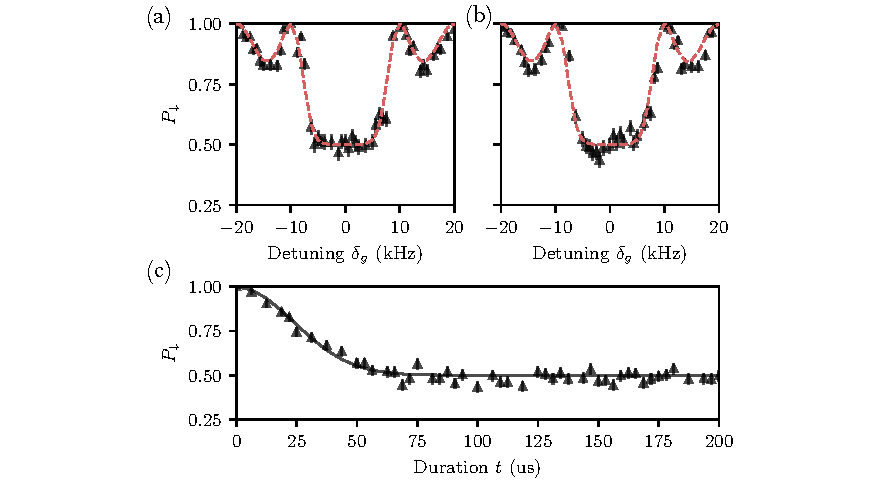
\includegraphics[width=\linewidth]{
            figures/pdf_figure/ch4/sdf.pdf
            }
        \end{center}
        \caption{
            Detuning and duration scans of the spin-dependent force applied to an initial thermal state with $\bar{n} = 0.03(1)$. 
            (a) Detuning scan, where the detuning, $\delta_g$, is varied, and the duration is fixed at $t=100$~\unit{\us}.  
            (b) Detuning scan with a mis-set qubit frequency of $0.5$~\unit{\kHz}. 
            (c) Duration scan, where the duration, $t$, is varied, and the detuning is fixed at $\delta_g = 0$. The solid line is a fit to the expected behaviour given by equation~\ref{eqn:sdf_pop} with only $\Omega_{\rm SDF}$ as a free parameter. The extracted $\Omega_{\rm SDF}$ is used with equation~\ref{eqn:sdf_pop} to plot the dashed red lines in (a) and (b) to guide the eye.
            }
        \label{fig:SDF}
    \end{figure}

    Spin-dependent forces (SDF), as described in~\S~\ref{sec:SDF}, are used in this thesis for both two-qubit entangling gates (following section), and for generating and characterising nonlinear bosonic states (~\S~\ref{sec:tomography} and \S~\ref{sec:two-sdf}). Here we describe the calibration strategy and characterisation of a single SDF.\\

    The SDF is generated using the bichromatic field method introduced by M{\o}lmer and S{\o}rensen~\cite{molmer_multiparticle_1999}, using simultaneous detuned red- and blue-sidebands.
    In practice, this SDF interaction involves relatively few degrees of freedom to calibrate:
    the central qubit ``carrier'' frequency, the motional mode frequency, the power in each
    optical tone, and ensuring negligible off-resonant excitation of other spin, and spin-motion interactions.\\

    The bichromatic field is generated by providing two simultaneous RF tones to the single-pass (SP) AOM, as seen in the \emph{TrapLab} panel of Figure~\ref{fig:729}. The SDF may be driven by either the single-ion addressing system (path 729\#1), or by a global field (path 729\#2). The SP AOMs are driven by an arbitrary waveform generator\footnote{\emph{Phaser Sinara} board} to provide phase, frequency, and amplitude control over the two tones.\\
    The bichromatic field is measured using a high-bandwidth photodiode after an optical pick-off before addressing the ions. The intensity measured by the photodiode has a beat-note with frequency $\omega_b \approx 2\omega_\mathrm{upper}$. The contrast of this beat-note is optimised to calibrate the power balance between the two optical frequencies. The power balance is varied by updating the RF amplitude supplied to the SP AOMs.
    AOMs generate frequency shifts in the laser beam at the expense of small
    frequency-dependent angular shifts. The beam pointing of the diffracted order also has some temperature dependence. After the AOM, the beam is coupled into a
    single mode fibre, as such the AOMs introduce a
    frequency- and temperature-dependent loss. These losses can lead to significant errors in power-balance between the two tones. We found that optimising for short optical path-lengths between the SP AOM and the fibre, careful alignment to the fibre, and ensuring the SP AOM is supplied with a constant duty cycle were all required for stable power-balance.\\
    Off-resonant excitations of other interactions are negated through selecting trap parameters to spectrally isolate a single-motional mode, and ensuring that gates are driven adiabatically --- the SDF Rabi frequency, $\Omega$, is significantly less than the frequency spacing to nearby interactions. Ensuring the interaction is smoothly ramped on and off also reduces excess off-resonant excitations.\\
    The bichromatic field leads to a Stark shift, $\delta_s$, of the central qubit frequency due to off-resonant coupling of both dipole and nearby quadrupole transitions. As such, the bare-qubit frequency measured by RPE in~\S~\ref{sec:RPE} is insufficient for low-error SDFs.
    The Stark-shift calibration is thus done through observing the application of the SDF to the ion when all other parameters are well calibrated.
    When the qubit frequency is set incorrectly, by $\Delta$, the two tones no
    longer have the same absolute detuning from their respective RSB or BSB. The impact of this error depends on the detuning of the SDF compared to the motional mode, $\delta_g$. When $\delta_g \gg \Delta$ the induced phase space dynamics are similar to the desired interaction, however when $\delta_g \approx \Delta$, we see a strong deviation from ideal behaviour due to the resonant driving of only one of the sidebands. We utilise this frequency dependent non-ideal behaviour of the uncalibrated SDF to manually calibrate the induced qubit Stark shift.  
    The phase space dynamics can be observed through projective spin measurements. 
    An SDF square pulse of duration $t_\mathrm{pulse}$ with spin conditioning, $\hat\sigma_x$, and variable detuning, $\delta_g$, is applied to the initial prepared state $\ket{\da,0}$.
    The spin population returns to $P_\da=1$ only when the pulse duration and SDF detuning are related by $\delta_g = \frac{2\pi}{nt_\mathrm{pulse}}$, for integer $n$. These spin dynamics are described by~\cite{burd_squeezing_nodate},
    \begin{equation}
        \label{eqn:sdf_pop}
        P_{\downarrow,\mathrm{th}} = \frac{1}{2} \left( 1 + e^{-4\left( \bar{n} + \frac{1}{2} \right) |\beta(t, \delta_g)|^2} \right),
    \end{equation}
    where $\bar{n}$ is the initial thermal phonon occupation, and $|\beta(t, \delta_g)| = \Omega_{\rm SDF} \sin(\delta_g t/2)/\delta_g$, is the absolute displacement of the initial state. Deviations from this behaviour indicate either a miscalibration of Stark shift, or unintended off-resonant excitation of nearby transitions.\\
    To give an example of this calibration procedure we show experimental data of both a well-calibrated, and a miscalibrated SDF, in Figure~\ref{fig:SDF}~(a), and (b) respectively. For these detuning scans we set $t_\mathrm{pulse}=100~\unit{\micro\second}$, and use the global addressing beam with $2~\unit{\milli\watt}$ of total power. The points indicate the spin population averaged from 200 samples. The calibrated scan assumes a Stark-shift $\delta_s=2\pi\times4\unit{\kilo\hertz}$, while the miscalibrated scan assumes $\delta_s=2\pi\times3.5\unit{\kilo\hertz}$.
    The dashed red lines in both (a) and (b) are the expected population dynamics inferred using an independently measured SDF strength of $\Omega_{\rm SDF}$. The well-calibrated SDF shows good agreement to the expected dynamics, while the qubit-frequency mis-calibrated SDF displays a clear asymmetry near $\delta_g=0$.\\
    Panel (c) displays a ``splitting'' experiment, applying the SDF on resonance $\delta_g = 0$, and varying the duration. The solid black line is a fit of the spin populations using equation~\ref{eqn:sdf_pop}, and assuming $\bar{n}=0$. We find here $\Omega_\mathrm{SDF}=2\pi\times6.6(2)~\unit{\kilo\hertz}$. Splitting of the motional wave-packet by a resonant SDF is exactly the procedure used for motional state tomography, which we give further details for in~\S~\ref{sec:tomography}.
    

\subsection{Two-Qubit Entangling Gates}
\label{sec:Two-Qubit Entangling Gates}
% Main points:
    % Intro/brief outline of goal of two-qubit gate. Truth table? Preparing in Bell state. This is tool kit for spin control of our system.
    % Discuss likely limitations being nearby hot motional modes, no pulse ramping
    % Current error vs what we expect we need for future experiments.
    % Here empasise that the SDF we discuss previously can be used to generate entanglement.
    % Showing phase coherence between operations is nice here.
% Prereqs:
    % SDFs
    % Single qubit gates
    % What available transitions we have
    % Motional mode spectra

    \begin{figure}
        \begin{center}
        \noindent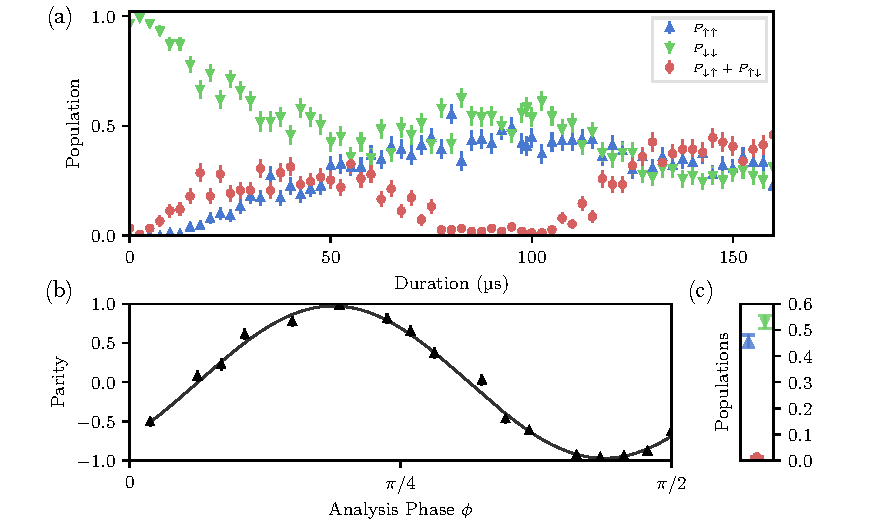
\includegraphics[width=\linewidth]{
            figures/pdf_figure/ch4/ms_walsh.pdf
            }
        \end{center}
        \caption{
            Experimental calibration and characterisation of a Walsh-modulated Mølmer-Sørensen (MS) two-qubit entangling gate with fidelity $\mathcal{F}=0.980(6)$.
            (a) Populations versus duration scan of the MS interaction.
            Each point corresponds to the average of 200 shots, and the error
            bars are given by the standard deviation of these averages. The desired
            entangling gate corresponds here to $t_g =  95$\unit{\us}. 
            (b) Observed parity oscillations after the MS interaction. The fitted
            contrast here is $C=0.97(1)$.
            (c) Populations at the desired entangling gate duration, $t_g =
            95$~\unit{us}.  
            }
        \label{fig:ms_gate}
    \end{figure}

    To complete the demonstration of elementary operations required for
    universal qubit control, we characterise the performance of two-qubit
    entangling gates, $R_{xx}(\theta)$, via the MS interaction on our apparatus.\\
    This interaction, as discuss in~\S~\ref{sec:Geometric Phase Gates}, is
    implemented through a detuned SDF.
    To reduce the sensitivity to incoherent motional errors such as heating and dephasing, a multi-loop 
    sequence is used. Specifically, we use a ``Walsh-modulated two-loop'' sequence consisting of two complete loops in phase space with the motional phase of the SDF flipped by $\pi$ for the second loop~\cite{hayes_coherent_2012}. The two-loop gate requires
    gate duration and detuning related by
    equation~\ref{eqn:nloop}, yielding, $T_2 = \frac{\pi\sqrt{2}}{\Omega_{\rm
    SDF}}$ and $\delta_g = 2\sqrt{2}\Omega_{\rm SDF}$. The 
    change of SDF sign after the first loop reduces sensitivity to
    systematic detuning offsets, for example due to mode-frequency drift.

    The two-qubit gate performance can be characterised many different ways.
    Ideally a process tomography method would be used to fully characterise the
    CPTP map implemented by the noisy two-qubit
    gate~\cite{chuang_prescription_1997}. However such a method requires
    near-perfect state-initialisation to correctly discern dynamics originating
    from the gate under test. Random circuit methods such as two-qubit Clifford
    RB~\cite{gaebler_randomized_2012}, or cyclic
    benchmarking~\cite{erhard_characterizing_2019} could also be used to gain
    single-value performance metrics insensitive to state-preparation errors. In
    this thesis we use a state tomographic
    technique~\cite{sackett_experimental_2000}, which although does not
    rigorously characterise the action of the gate on arbitrary initial states,
    is quick to implement, and only requires a single additional
    $R_x(\frac{\pi}{2})$-pulse.\\
    A single $R_{\phi_s\phi_s}(\frac{\pi}{2})$ two-qubit entangling gate, where
    $\phi_s$ is some fixed angle in the $xy$-plane, is applied to the initial
    state $\ket{\da\da}$. This gate targets the creation of the 
    maximally-entangled state $\ket{\Phi^+_{\phi_0}} = 1/\sqrt{2} \left( \ket{\downarrow\downarrow} +
    e^{i\phi_0}\ket{\uparrow\uparrow} \right)$, where $\phi_0$, is some fixed
    phase\footnote{$\phi_0$ is left unspecified as the target of a specific
    phase is not required, we only require that it is stable over time, and
    measured precisely.}. Practically, due to systematic errors and noise on
    both the qubit and motional state, the final mixed state $\hat\rho$ is produced.
    The state-fidelity between $\hat\rho$, and the pure Bell state is
    given by,
    \begin{equation}
        \mathcal{F} = \bra{\Phi^+_{\phi_0}} \hat\rho \ket{\Phi^+_{\phi_0}} = \frac{1}{2} \left( \rho_{\da\da,\da\da} + \rho_{\ua\ua,\ua\ua} \right) + \frac{1}{2}\left( e^{i\phi_0}\rho_{\ua\ua,\da\da}+e^{-i\phi_0}\rho_{\da\da,\ua\ua}\right),
        \label{eq:Fidelity}
    \end{equation}
    where the matrix elements are given by $\rho_{ij,kl} = \braket{ij|\hat\rho|kl}$.
    Thus to extract this fidelity, only partial state tomography is
    required~\cite{sackett_experimental_2000}.
    The first bracketed term of
    equation~\ref{eq:Fidelity}, denoted $A$, is measured by performing projective measurements
    of the two ions after the applied $R_{\phi_s\phi_s}(\frac{\pi}{2})$. The extracted
    two-qubit joint populations directly recover this population term, $A=
    P_{\da\da} + P_{\ua\ua}$, where $P_{ij}$ is the population of the two ions
    in state $\ket{i}\ket{j}$.
    The coherence terms in the second bracket are measured by applying a global analysis
    $R_\phi(\pi/2)$ pulse to the two ions with variable phase $\phi$. The final
    spin populations are combined to a parity measurement, defined as $\Pi =
    P_{\da\da} + P_{\ua\ua} - P_{\da\ua} - P_{\ua\da}$. Varying $\phi$, the
    observed parity relates to the matrix elements of $\hat\rho$ as,
    \begin{equation}
        \Pi(\phi) = \rho_{\da\ua,\ua\da}+\rho_{\ua\da,\da\ua} + e^{-2i\phi}\rho_{\ua\ua,\da\da} + e^{+2i\phi}\rho_{\da\da,\ua\ua}.
    \end{equation}
    In the case that there are no coherences between single-excitation states
    $\ket{01}\leftrightarrow\ket{10}$, the parity reduces to simple oscillations
    of the form,
    \begin{equation}
        \Pi(\phi) =  2\mathrm{Re}\left[e^{-2i\phi}e^{i\phi_0}|\rho_{\ua\ua,\da\da}|\right]=C\cos(2\phi-\phi_0),
    \end{equation}
    where we have taken $\rho_{\ua\ua,\da\da} :=
    e^{i\phi_0}|\rho_{\ua\ua,\da\da}|$, and $C=2|\rho_{\ua\ua,\da\da}|$. The
    contrast of the parity oscillations thus provide the magnitude of the
    coherence term.
    The Bell-state fidelity is thus given by $\mathcal{F} = \frac{A + C}{2}$.\\

    Using this method, the fidelity of a globally addressed two-qubit entangling
    gate by the Walsh method is experimentally measured.
    Figure~\ref{fig:ms_gate} (a) shows the spin-population dynamics as a
    function of total Walsh-1 duration for an MS gate acting on the upper radial
    common mode, with gate parameters, $\delta_g = -19.5~\unit{\kilo\hertz}$, and
    $35~\unit{\milli\watt}$ of total beam power, causing a Stark shift of
    $\delta_s=14~\unit{\kilo\hertz}$. To suppress off-resonant excitation of
    nearby spin-motion interactions, the SDF field is ramped on and off with a
    rise envelope of $\sin^2(\pi t/(2t_\mathrm{ramp}))$ applied via the AWG, where
    $t_\mathrm{ramp}=9.6~\unit{\micro\second}$ is the ramp duration. The desired
    geometric phase is accumulated by $t_g=95~\unit{\micro\second}$. The parity
    oscillations and two-qubit populations are measured at this point, and shown
    in panels (b) and (c) respectively. A contrast of $C=0.97(1)$, and
    population of $A=0.987(2)$ is found, resulting in a state fidelity,
    $\mathcal{F}=0.980(6)$.
    Each population point in these figures are found by taking the
    average of 200 shots of the gate sequence.\\
    Similar fidelities were measured when applying the interaction by the single-ion addressing system on
    the upper radial common mode. Using
    gate parameters $\delta_g = -15~\unit{\kilo\hertz}$, $t_g=110~\unit{\micro\second}$, and
    $0.148~\unit{\milli\watt}$ of total beam power,
    a fidelity of
    $\mathcal{F}=0.983(4)$ was measured, with contrast $C=0.976(7)$ and
    population contribution $A=0.991(1)$.\\

    We believe we are currently limited either by systematic calibration errors,
    or by laser phase noise of the 729-nm system. We have anecdotally observed a
    strong dependence on the gate-fidelity with PID parameters for the 729-nm
    PDH lock. To increase the two-qubit gate fidelity, we believe that further time
    must be devoted to characterising the noise-spectrum of the 729-nm, and
    optimising lock parameters to suppress phase noise at the frequencies
    relevant to the two-qubit entangling gates. This, along with developing an
    automated gate-tuning algorithm for our apparatus, is left to future work.
    The current fidelities observed here are sufficient for the projects outlined in this
    thesis. In~\S~\ref{sec:vd_exp} we calibrate $R_{xx}(\frac{\pi}{4})$ gates
    using this state-fidelity approach.

\begin{table}[]
    \centering
    \begin{tabular}{c|c|c}
         Operation & Fidelity & Section \\
         \hline\hline
         State Prep &99.96(2)& \S~\ref{sec:Stateprep}\\
         Measurement &$ < 99.7(3)$& \S~\ref{sec:standard_rb}\\
         $R_x(\pi/2)$ & 99.913(2) & \S~\ref{sec:standard_rb}\\
         $R_{xx}(\pi/2)$ & 98.3(4) & \S~\ref{sec:Two-Qubit Entangling Gates}\\
    \end{tabular}
    \caption{
        Summary of qubit-operation fidelities presented in this chapter.
    }
    \label{tab:fidelities}
\end{table}
\section{Summary}
    These results serve as both a proof of principle for full discrete-variable control on
    our system, but also as a benchmark to which we can compare future system
    improvements. The fidelities of the operations demonstrated in this chapter are summarised in Table~\ref{tab:fidelities}, with relevant sections highlighted.

    